% BAC 2024 D - Exercice 3
% Courbe de f(x) = x - 3 + (1/2)e^x
% Asymptote oblique D: y = x - 3

\documentclass[border=5pt]{standalone}
\usepackage{pgfplots}
\usepackage{amsmath}
\usepackage{amssymb}

\begin{document}

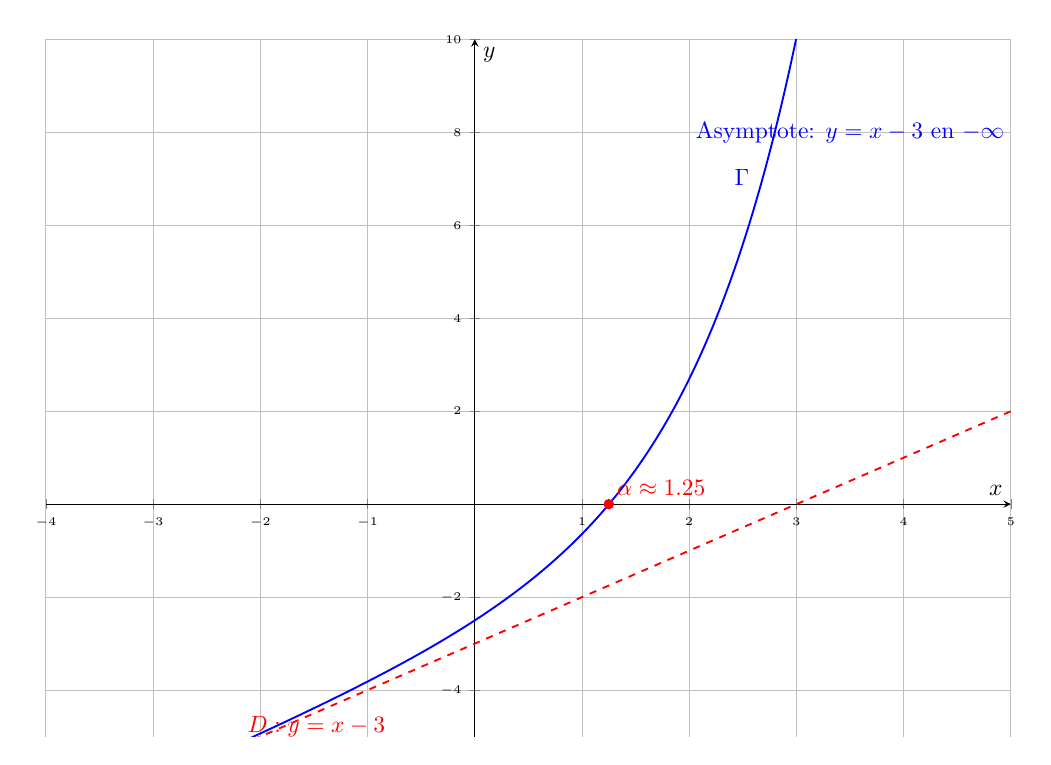
\begin{tikzpicture}[scale=0.85]
\begin{axis}[
    width=16cm,
    height=12cm,
    axis lines=center,
    xlabel=$x$,
    ylabel=$y$,
    xmin=-4, xmax=5,
    ymin=-5, ymax=10,
    grid=major,
    samples=200,
    legend pos=outer north east,
    tick label style={font=\tiny}
]

% Function f(x) = x - 3 + 0.5*e^x
\addplot[blue, thick, domain=-4:3.5] {x - 3 + 0.5*exp(x)} 
    node[pos=0.6, above left] {$\Gamma$};

% Asymptote oblique D: y = x - 3
\addplot[red, dashed, thick, domain=-4:5] {x - 3} 
    node[pos=0.2, above right] {$D: y = x - 3$};

% Point alpha (solution de f(x)=0, environ 1.2-1.3)
\addplot[mark=*, red] coordinates {(1.25, 0)} 
    node[above right] {$\alpha \approx 1.25$};

% Annotation: tangente en +∞
\node[blue] at (3.5,8) {Asymptote: $y = x - 3$ en $-\infty$};

% Vertical asymptote n'existe pas
% La fonction est définie sur tout R

\end{axis}

\end{tikzpicture}

\end{document}